\subsection{Annealing based alternating optimization (AAO) for proximity and diversity maximization}
\label{sec:aao}
In this section, we describe an approach where two iterative algorithms, each optimizing for a certain objective function, are run alternately in order to obtain a solution that is a mutual trade-off between the two objectives. The two algorithms have the task of selecting a set of $L$ keywords amongst the valid keywords, such that the selected set maximizes average proximity and diversity respectively. The algorithms are discussed in detail in Sections~\ref{sec:aaoproxmax} and \ref{sec:aaodivmax} respectively. The methodology adopted for measuring average proximity and diversity of the set of selected keywords for the purpose of this approach is described next.  

\subsubsection{Measurement of proximity and diversity scores}
\label{sec:proxdivmeasureAAO}

For the AAO approach, proximity of a keyword $K$ is measured as detailed in Section~\ref{sec:overviewselectSRK}. For the LCPD approach, diversity was measured as the variance of the set of videos retrieved. Based on this, a diversity score per keyword given a training data was defined (\ref{eq:divscorelcpd}). Such a measurement was feasible for LCPD as it does not need to employ an algorithm to maximize the diversity of a set of keywords. In contrast to LCPD, the AAO approach measures diversity for a set of keywords, and not per keyword given certain training data. Using such a diversity measure, AAO employs an efficient algorithm capable of selecting the set of $L$ keywords that has the maximum diversity. In order to define diversity for a set of keywords, we first represent each keyword $K$ by the centroid of its retrieved videos $RV(K)$. The diversity of a set of keywords could be defined based on certain pair-wise distances measures between the keywords, however an optimization technique based on such a measure would essentially boil down to performing a combinatorial search over all $L$-sized subsets of the set of valid keywords, making it highly inefficient if not infeasible. As an example, for selecting 25 keywords from 200 valid keywords, this means going through ${200 \choose 25}$ i.e., around $4*10^{31}$ subsets. Hence, for AAO we develop a different way of measuring diversity: the diversity of a set of keywords is defined based on the degree of linear independence between the keywords. Doing so leads to highly efficient optimization through Rank-Revealing QR (RR-QR) factorizations, to obtain which efficient algorithms have been proposed in literature \cite{BusingerLinear65,GolubNumeri65,ChanRank87,GuEfficient96}. 

Assume that the set of $L$ keywords for which we would like to calculate the diversity is $x_L = \{K_j\}$ where $j$ = $1$ to $L$. The matrix representation of $x_L$ is $X_L \in \mathbb{R} ^{m\times L} $ where $m$ is the dimensionality of the representation of each video i.e., the size of the bag of words representation of each video, and $m \ge L$. The $j^{th}$ column of $X_L$ is represented as $\mu_{Kj}$ i.e., as the centroid of the set of videos RV($K_j$). The \textbf{diversity score} of the set of keywords $x_L$ is then defined as 
\begin{equation} \label{eq:divaao}
\text{Diversity score for $x_L$}=\prod_{b}{\sigma_b(X_L) }, 
\end{equation}
 where $\sigma_b(X_L)$ is the $b^{th}$ singular value of the matrix $X_L$. 

\subsubsection{Overall Approach for AAO}
\label{sec:overallAAO}

The AAO approach optimizes for two objectives (average proximity score, and diversity score of a set of keywords) alternately, under a simulated annealing framework. Average proximity score of a set of keywords, as the name implies, is the average of the proximity scores of the keywords in the set. This is represented as $O_{Proximity}$. Diversity score of a set of keywords is represented as $O_{Diversity}$ and is calculated using~(\ref{eq:divaao}). The two iterative algorithms that optimize for these objective functions individually can converge to the most proximate or the most diverse set of keywords respectively. However, we add a constraint parameter $T$ where $T \in \lbrack 1, \infty)$ in the framework that controls the extent to which each algorithm is permitted to run. The individual optimization algorithms are such that $T$ can be provided as an input. They also take a set of keywords as input for the initial solution and improve the solution in each iteration. For a lenient (lower) value of $T$, either of the algorithms is permitted to run for more number of iterations and as a result, the solution at the end of the run is better in terms of the corresponding objective function. The constraint parameter $T$ is set to $1$ to start with, which allows both algorithms to optimize for their respective objective functions. 

\begin{figure}
\centering
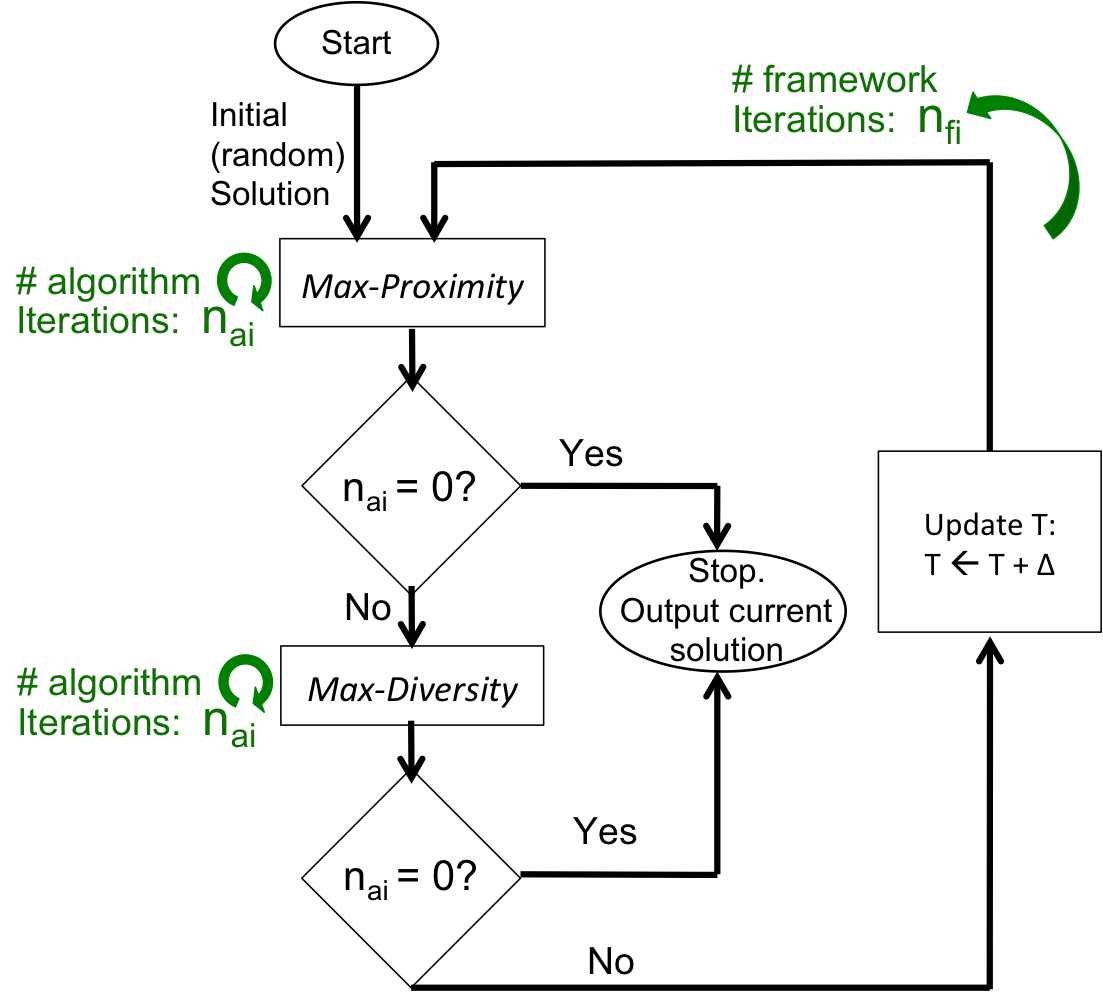
\includegraphics[width=0.75\linewidth]{TrainingData/figs/aao_overview.png}
\caption{Overview of the AAO approach for alternately optimizing the average proximity and diversity of selected keywords}
\label{fig:AAOoverview}
\end{figure}

Fig.~\ref{fig:AAOoverview} gives an overview of the AAO approach. The iterative algorithm to optimize for $O_{Proximity}$ (shown as \textit{Max-Proximity} in Fig.~\ref{fig:AAOoverview}) is initially run based on a random set of $L$ keywords and $T=1$, and selects the set of $L$ keywords that has the highest average proximity. This set is provided as input to the iterative algorithm to optimize for $O_{Diversity}$ (shown as \textit{Max-Diversity} in Fig.~\ref{fig:AAOoverview}), along with the same value of $T$. This leads to the selection of a set of $L$ keywords having the maximum diversity score. This completes the first iteration of the AAO framework, also referred to as the first \textbf{framework iteration}. Framework iterations are represented by $n_{fi}$. For 20 valid candidate keywords of the category Baby and for $T=1$, the sets of 5 keywords obtained at the end of either algorithm are provided in Figures~\ref{fig:proxdivkwdBabyExamplePCA}(a) and \ref{fig:proxdivkwdBabyExamplePCA}(b) respectively. The output, i.e., the set of keywords selected at the end of the first framework iteration is then routed back to the \textit{Max-Proximity} algorithm to start the second framework iteration. At this point, the constraint parameter $T$ is increased by a constant amount $\Delta$ to a higher and thus a stricter value. As a result of the stricter value of $T$, the algorithm \textit{Max-Proximity} is constrained from running completely. While it may select a set of keywords with higher average proximity than the output of first framework iteration, the set of keywords selected may not maximize the average proximity as the algorithm was prevented from running completely. This process continues and the value of $T$ is increased at the end of each framework iteration, thus making it harder for the algorithms to select keywords that maximize their corresponding objective functions. The framework stops when either of the two algorithms cannot proceed. 

The sets of selected keywords obtained at the end of the algorithms \textit{Max-Proximity} and \textit{Max-Diversity} vary a lot with each other in the initial framework iterations. This can be seen in Fig.~\ref{fig:proxdivVariationAAO}(b) where a higher intensity of colors (red or blue) reflects a higher value of the corresponding objective function (average proximity or diversity respectively). As $T$ increases, the variation in the outputs at the end of the two algorithms reduces. The overall annealing based optimization framework is detailed in Algorithm II. Note that the overall framework is iterative and the individual algorithms that maximize average proximity or diversity are iterative too. In order to avoid confusion, an iteration of either \textit{Max-Proximity} algorithm, or of \textit{Max-Diversity} algorithm is referred to as an \textbf{algorithm iteration} and is represented by $n_{ai}$. Details on the individual iterative algorithms that optimize for the two objective functions are provided in the next section. Note that the proof of convergence for Algorithm II is given after describing \textit{Max-Proximity} and \textit{Max-Diversity} algorithms since the proof requires convergence properties of \textit{Max-Proximity}. 

In Section~\ref{sec:adaptAAO} we study the effect of $\Delta$ on the convergence of the AAO framework, specifically on the resulting set of keywords after convergence and on the time taken to converge. Further, in order to reduce the time taken by the optimization framework to converge without inducing bias in the end result, we propose an adaptive technique to update the constraint parameter $T$ based on the \textit{weakest permitted} algorithm iteration of the previous framework iteration. Details and the definition of the weakest permitted algorithm iteration are provided in Section~\ref{sec:adaptAAO}. 

\begin{algorithm}
\fontsize{8pt}{1em}\selectfont
\caption{Annealing based alternating optimization (AAO) framework for maximizing average proximity and diversity of selected keywords}
\label{algo:AAO}
\textbf{Inputs:} \\ 
\hspace*{2mm}          Number of keywords: $L$ \\ 
\hspace*{2mm}          Set of valid keywords: $K_{Valid}$ \\
\hspace*{2mm}          Representation of valid keywords in matrix form: $X$ \\
\hspace*{2mm}          Proximity score $\forall K \in K_{Valid}$ \\
\hspace*{2mm}          Increment for constraint parameter ($T$): $\Delta$ \\ 	
\hspace*{2mm}   (Note that the subscript $i$ is dropped since the algorithm is  \\ 
\hspace*{2mm}   run for each category separately) \\ 
\textbf{Initialization:} \\ 
\hspace*{2mm}       $K_{SRK}$ $\leftarrow$ set of random $L$ keywords from $K_{Valid}$\\ 
\hspace*{2mm}          $T \leftarrow 1$ \\ 
\hspace*{2mm}          $n_{fi} \leftarrow 0$  \\ 
\textbf{Begin framework iterations: } \\ 
\hspace*{2mm}       While (1) 		 \\ 
\hspace*{6mm}        \textbf{Maximize proximity:} \\ 
\hspace*{6mm}        ($K_{SRK}$, $n_{ai}$) $\leftarrow$ \textit{Max-Proximity}($K_{SRK}$, $T$, Proximity scores) \,\,\,\,\,\,\,\,\,\,\,\,\,\,\,\,\,\,\,\,\,\,\,\,\,\\
\hspace*{6mm}        If ($n_{ai} = 0$):  STOP \\
\hspace*{6mm}        \textbf{Maximize diversity: } \\ 
\hspace*{6mm}        ($K_{SRK}$, $n_{ai}$) $\leftarrow$ \textit{Max-Diversity}($K_{SRK}$, $T$, $X$) \\
\hspace*{6mm}        If ($n_{ai} = 0$):  STOP    \\ 
\hspace*{6mm}        $T \leftarrow T + \Delta$ (increment constraint parameter) \\ 
\hspace*{6mm}        $n_{fi} \leftarrow n_{fi} + 1 $ \\ 
\hspace*{2mm}       End While \\ 
\textbf{Output:} Selected set of retriever keywords: $K_{SRK} $  
\end{algorithm}




\begin{algorithm}
\fontsize{8pt}{1em}\selectfont
\caption{Max-Proximity algorithm}
\label{algo:maxproximity}
\textbf{Inputs:}  \\ 
\hspace*{2mm}   Initial set of selected keywords: $I_{SRK}$ \\ 
\hspace*{2mm}   Constraint parameter: $T$ \\ 
\hspace*{2mm}   Valid keywords $K_{Valid}$ and Proximity score $\forall K \in  K_{Valid}$ \\ %  as Proximity($K$)  \\ 
\hspace*{2mm}   (Note that the subscript $i$ is dropped since the algorithm is \\ 
\hspace*{2mm}   run for each category separately) \\ 
\textbf{Initialization:} \\ 
\hspace*{2mm}  $L \leftarrow \mid I_{SRK} \mid$ \\ 
\hspace*{2mm}   $K_{SRK} \leftarrow I_{SRK} $ \\   
\hspace*{2mm}   $WI_{Proximity} \leftarrow$ an arbitrarily large value \\ 
\hspace*{2mm}   ($WI_{Proximity}$: Weakest permitted algorithm iteration) \\ 
\hspace*{2mm}   $n_{ai} \leftarrow 0$ \\ 
\textbf{Begin framework iterations: } \\ 
\hspace*{2mm} While (1) 		 \\ 
\hspace*{6mm}        $O_{Proximity} \leftarrow $ Average proximity score of $K_{SRK}$ \\       
\hspace*{6mm}               Replace least proximate keyword in $K_{SRK}$ with most proximate keyword in \{$K_{Valid} \setminus K_{SRK}$\} to get $K\text{'}_{SRK}$  \\ 
\hspace*{6mm}               $O\text{'}_{Proximity} \leftarrow$ Average proximity score of $K\text{'}_{SRK}$ \\  
\hspace*{6mm}               If $\frac{O\text{'}_{Proximity}}{O_{Proximity}} > T$: \\ 
\hspace*{10mm}               $K_{SRK} \leftarrow K\text{'}_{SRK}$ \\ 
\hspace*{10mm}                           If $\frac{O\text{'}_{Proximity}}{O_{Proximity}}  < WI_{Proximity}$:\\ 
\hspace*{14mm}        	         $WI_{Proximity} \leftarrow \frac{O\text{'}_{Proximity}}{O_{Proximity}} $ \\ 
\hspace*{6mm}               Else:  STOP \\  
\hspace*{6mm}        $n_{ai} \leftarrow n_{ai} + 1 $ \\ 
\hspace*{2mm} End While \\ 
\textbf{Outputs: } \\ 
\hspace*{2mm}Selected set of retriever keywords: $K_{SRK}$ \\ 
\hspace*{2mm}$WI_{Proximity}$ (useful for Algorithm \ref{algo:AdaptAAO}) \\
\hspace*{2mm}Number of algorithm iterations: $n_{ai}$
\end{algorithm}

\subsubsection{Average proximity score maximization }
\label{sec:aaoproxmax}

The proximity scores of valid keywords for a category are fixed values defined as per (\ref{eq:proximityscore}). The easiest way to maximize the average proximity of selected $L$ keywords from the set of valid keywords for category $i$, i.e., from $K_{Valid,i}$, is to select the $L$ keywords from $K_{Valid, i}$ having the highest proximity scores. However such an approach does not permit adding a constraint parameter ($T$) to control the extent to which the proximity maximization algorithm is run. In order to do that, we propose an iterative algorithm \textit{Max-Proximity} that maximizes the average proximity of selected $L$ keywords by performing exchanges or swaps between the selected keywords and the non-selected valid keywords. \textit{Max-Proximity} is presented in Algorithm~\ref{algo:maxproximity}. Each iteration of the algorithm checks if replacing the selected keyword having the least proximity score (i.e., the least proximate selected keyword) with the most proximate non-selected valid keyword leads to a \textit{relative benefit} in average proximity above the constraint parameter $T$. The relative benefit is defined as a ratio of the average proximity of the selected keywords after the swap, with the average proximity before the swap. If that is the case, the above mentioned two keywords are swapped and the set of selected keywords $K_{SRK,i}$ is updated. If not, the algorithm terminates since this means no other swap between the keywords would lead to a relative benefit in average proximity above $T$. The algorithm takes as input and starts from a set of $L$ keywords as $K_{SRK,i}$, referred to in Algorithm~\ref{algo:maxproximity} as $I$. When $T$ is equal to $1$, any improvement in the average proximity score is acceptable and \textit{Max-Proximity} converges to the set of $L$ keywords having highest proximity scores. 

\textbf{Proof of correctness for Algorithm~\ref{algo:maxproximity}. } 
%\begin{proof}
We prove that \textit{Max-Proximity} (Algorithm~\ref{algo:maxproximity}) leads to maximization of the average proximity score when permitted to run completely, i.e., when $T=1$. Assume that $S_{OptProx}$ is the optimal set of keywords that maximizes the average proximity score amongst a set of valid keywords $K_{Valid}$. $S_{OptProx}$ then comprises of the $L$ keywords in $K_{Valid}$ which have the highest proximity score. Also assume that $S_{init}$ is the set of valid keywords that are given as initialization to Algorithm~\ref{algo:maxproximity}. The cardinality of $S_{init}$ is $L$, the number of keywords that are to be selected by \textit{Max-Proximity}. Then, there are ($\mid S_{OptProx} \cap S_{init} \mid$) keywords in $S_{init}$ that are also in $S_{OptProx}$, and are also the ($\mid S_{OptProx} \cap S_{init} \mid$) most proximate keywords in $S_{init}$. In $\mid S_{OptProx} \setminus S_{init}  \mid$ iterations of Algorithm~\ref{algo:maxproximity}, the  $\mid S_{OptProx} \setminus S_{init} \mid$ least proximate keywords from $S_{init}$ will be exchanged (swapped) with the keywords in the set $S_{OptProx} \setminus S_{init}$ in the order of decreasing proximity score of the latter. All such exchanges replace a keyword having a lower proximity score with another having a higher proximity score. Thus, the average proximity score of the selected keywords goes up by some amount in each iteration and since $T=1$, any improvement would be acceptable. Thus, at the end of $\mid S_{OptProx} \setminus S_{init} \mid$ iterations, the set of keywords that will be selected will be $S_{OptProx}$. \hfill $\square$
%\end{proof}

As a corollary, since \textit{Max-Proximity} takes $\mid S_{OptProx} \setminus S_{init} \mid$ iterations to select the set of most proximate keywords, and since  $\mid S_{OptProx} \setminus S_{init} \mid$ can take a maximum value of $L$, the maximum number of iterations that \textit{Max-Proximity} can run for is $L$. 

\textbf{Complexity analysis for Algorithm~\ref{algo:maxproximity}.} The complexity of Algorithm~\ref{algo:maxproximity} per keyword exchange is $O(L (N_{Valid} -L))$ where $L$ is the number of SRKs. Since $N_{Valid} \ge L$, and the maximum number of algorithm iterations is $L$, the worst case complexity of Algorithm~\ref{algo:maxproximity} is $O(L^2 N_{Valid})$. 


\subsubsection{Diversity score maximization}
\label{sec:aaodivmax}
\begin{algorithm}
\fontsize{8pt}{1em}\selectfont
\caption{Max-Diversity algorithm }
\label{algo:maxdiversity}
\textbf{Inputs:}  \\ 
\hspace*{2mm}   Initial set of selected keywords: $I_{SRK}$ \\ 
\hspace*{2mm}   Constraint parameter: $T$ \\ 
\hspace*{2mm}   Valid keywords $K_{Valid}$ and their matrix form: $X$ \\ 
%\hspace*{2mm}    corresponding to the set $K_{Valid}$ \\ 
\hspace*{2mm}   (Note that the subscript $i$ is dropped since the algorithm is  \\ 
\hspace*{2mm}   run for each category separately) \\ 
\textbf{Initialization:} \\ 
\hspace*{2mm}   $L \leftarrow \mid I_{SRK} \mid$ \\ 
\hspace*{2mm}   $K_{SRK} \leftarrow I_{SRK} $ \\   
\hspace*{2mm}   Obtain $\Pi_{init}$ such that keywords in $K_{SRK}$ are the \\
\hspace*{2mm}   first $L$ columns of $X$ \\ 
\hspace*{2mm}   $X \leftarrow X \Pi_{init} $ (rearrange columns of $X$)  \\ 
\hspace*{2mm}   $WI_{Diversity} \leftarrow $ an arbitrarily large value \\ 
\hspace*{2mm}   ($WI_{Diversity}$: Weakest permitted algorithm iteration) \\ 
\hspace*{2mm}   $n_{ai} \leftarrow 0$ \\ 
\textbf{Begin framework iterations: } \\ 
\hspace*{2mm}   While (1) 		 \\ 
\hspace*{6mm}        Compute QR factorization of X to get $A_L$, $B_L$, $C_L$ \\ 
\hspace*{6mm}        as per (\ref{eq:rrqr})  \\ 
\hspace*{6mm}        Calculate $G_{i,j}$ as: 
\begin{equation}
G_{i,j} = \sqrt{  ( A_L^{-1} B_L )^2 _{i,j}   + (\frac{\gamma_j(C_L)}{w_i(A_L)}  )^2 } 
\end{equation}

\hspace*{6mm}        Obtain the best swap as: $(\hat{i}, \hat{j}) \leftarrow \argmax_{i,j}{G_{i,j}}$ \\ 
\hspace*{6mm}        If $G_{\hat{i}, \hat{j}} > T$: \\ 
\hspace*{10mm}                           Update $K_{SRK}$: Replace $\hat{i}^{th}$ keyword of $K_{SRK}$ \\
\hspace*{10mm}                           with $\hat{j}^{th}$ keyword of $K_{Valid}  \setminus K_{SRK}$ \\ 
\hspace*{10mm}                           $X \leftarrow X \Pi_{ \hat{i} \leftrightarrow (\hat{j} + L) }$ \\ 
\hspace*{10mm}                           If $G_{ \hat{i}, \hat{j} }  < WI_{Diversity}$:  $WI_{Diversity} = G_{\hat{i}, \hat{j} }$ \\ 
\hspace*{6mm}               Else:  STOP \\ 
\hspace*{6mm}        $n_{ai} \leftarrow n_{ai} + 1 $ \\ 
\hspace*{2mm}   End While \\ 
\textbf{Outputs: }  \\ 
\hspace*{2mm}   Selected set of retriever keywords: $K_{SRK}$ \\ 
\hspace*{2mm}   $WI_{Diversity}$ (useful for Algorithm \ref{algo:AdaptAAO}) \\
\hspace*{2mm}   Number of algorithm iterations: $n_{ai}$
\end{algorithm}
We propose to use Rank Revealing QR factorization (RRQR) \cite{GuEfficient96} to select keywords having the highest diversity, where diversity of a set of keywords is measured using (\ref{eq:divaao}), since there exist efficient algorithms to provide RRQR factorization \cite{GuEfficient96,GolubNumeri65}. RRQR factorization has also been used in \cite{ShroffManifold11} to obtain diverse video frames for the application of video summarization. Let $x_i$ be the set of valid candidate keywords for category $i$. The discussion in this section is for a fixed category (category $i$) and so the subscript $i$ is dropped for convenience. Thus the set of valid keywords is represented as $X = \{K_j\}$ where $j$ = $1$ to $N_{Valid}$. As mentioned in Section~\ref{sec:proxdivmeasureAAO}, the matrix representation of $x$ is $X \in \mathbb{R}^{m\times N_{Valid}}$ where $m$ is the number of dimensions used to represent each valid keyword  and $m \ge N_{Valid}$. In order to describe the algorithm used to select the $L$ keywords from $x$ that maximize diversity, we first provide a brief discussion on RRQR factorization \cite{GuEfficient96,GolubNumeri65} and its objectives. 

Given a matrix $X \in \mathbb{R}^{a\times b}$ where $a \ge b$, consider the partial QR factorization of the form

\begin{equation} \label{eq:rrqr}
X \Pi = Q R = Q \bigl(\begin{smallmatrix}
A_L & B_L\\ 
 & C_L
\end{smallmatrix}\bigr),  
\end{equation}
where $Q \in \mathbb{R}^{a\times a}$ is an orthogonal matrix with nonnegative diagonal elements, $A_L \in \mathbb{R}^{L\times L}$ is an upper triangular matrix, $B_L \in \mathbb{R}^{L\times (b-L)}$ and $C_L \in \mathbb{R}^{(a-L)\times (b-L)}$. $\Pi \in \mathbb{R}^{b\times b}$ is a permutation matrix that is a square binary matrix having exactly one $1$ in each row and each column and $0$ everywhere else. $\Pi$ represents a specific permutation of the columns of the matrix $X$ and the permuted matrix can be obtained as $X \Pi$. For a given permutation $\Pi$, $X \Pi$ can be written as ($X_L$  $X_{(b-L)}$) where $X_L \in \mathbb{R}^{a\times L}$ is the matrix formed by the first $L$ columns of $X$, and $X_{(b-L)} \in \mathbb{R}^{a\times (b-L)}$ is the matrix formed by the last ($b-L$) columns of $X$. The degree of linear independence of the first $L$ columns of $X \Pi$ can be obtained as the determinant of the matrix $A_L$, also equal to the product of the singular values of the matrix $X_L$, i.e., $\prod_{j}{\sigma_j(X_L) }$. RRQR factorization aims to find the permutation $\Pi$ such that $X \Pi $ = ($X_L$  $X_{(b-L)}$) reveals the rank of the matrix $X$. This permutation $\Pi$ provides $X_L$ the $L$ most linearly independent columns of $X$. RRQR factorization does so by seeking $\Pi$ which maximizes the product of singular values of $X_L$. Please refer to \cite{BusingerLinear65,GolubNumeri65,ChanRank87,GuEfficient96} for further details and for proof of correctness of RRQR factorization. 

In order to adopt RRQR for AAO approach, we need to add a constraint on the RRQR algorithm based on the parameter $T$. Hence, in each algorithm iteration of RRQR, the \textit{relative benefit} is defined as the ratio of new and previous objective functions. The relative benefit is compared with $T$ to determine if the updated set of keywords is acceptable or not (Algorithm~\ref{algo:maxdiversity}). This ratio is represented as $G_{i,j}$ in Algorithm~\ref{algo:maxdiversity}. Since $T \ge 1$, this ensures that within a framework iteration of AAO, the diversity only increases with each algorithm iterations of RRQR algorithm. Note that in Algorithm~\ref{algo:maxdiversity}, for a non-singular matrix $W \in \mathbb{R}^{L\times L}$, $1/w_i(W)$ denotes the 2-norm of the $i^{th}$ row of $W^{-1}$. Also, for a matrix $W\text{'}$ with $L$ columns, $\gamma_j(W\text{'})$ denotes the 2-norm of the $j^{th}$ column of $W\text{'}$. 

\textbf{Complexity analysis for Algorithm~\ref{algo:maxdiversity}.} Using results from \cite{GuEfficient96}, the worst case time taken by Algorithm~\ref{algo:maxdiversity} is $O(mLN_{Valid})$ where $m$ is the number of dimensions used to represent each valid keyword. 

\textbf{Proof of convergence for Algorithm~\ref{algo:AAO}.}
Algorithm~\ref{algo:AAO} calls \textit{Max-Proximity} with an input set of $L$ keywords. We will first show that if the constraint parameter $T$ is increased beyond a value, $T_{MaxGainProx}$, then no iteration of \textit{Max-Proximity} can take place. Let $K_{LowP}$ and $K_{HighP}$ be distinct valid keywords with lowest and highest proximity score respectively. Let $S$' represent certain set of $L-1$ distinct valid keywords, and let $S$ represent the set of selected keywords in an iteration of \textit{Max-Proximity}, such that $S = S\text{'} \cup K_{LowP}$ and $K_{HighP} \not\in S$. The maximum relative gain in the average proximity score of selected keywords by exchanging one keyword would be when $K_{LowP}$ is replaced with $K_{HighP}$. Thus, the maximum relative change in the average proximity score of selected keywords can be $\frac{ Pr(K_{HighP}) + Pr(S\text{'})} { Pr(K_{LowP}) + Pr(S\text{'}) }$, i.e., equal to ($1  +  \frac{ K_{HighP} - K_{LowP}}{ Pr(K_{LowP}) + Pr(S\text{'}) }$). Here $Pr(K)$ and $Pr(S\text{'})$ refer to the proximity score of $K$ and the sum of proximity scores of the keywords in $S\text{'}$ respectively. The relative change is maximum when $S\text{'}$ corresponds to the $L$ least proximate keywords amongst valid keywords, except $K_{LowP}$. Let this value of the maximum relative change in average proximity be $T_{MaxGainProx}$. If $T > T_{MaxGainProx}$, then \textit{Max-Proximity} cannot run for any iteration because the relative gain in the average proximity score of selected keywords cannot exceed $T_{MaxGainProx}$. Thus, as per Algorithm~\ref{algo:AAO} when $T > T_{MaxGainProx}$, the AAO framework will stop. If the value of $\Delta$ is kept constant, the number of framework iterations it takes for $T$ to increase from $1$ to $T_{MaxGainProx}$ is $\left \lceil{ \frac{T_{MaxGainProx} -1}{\Delta} }\right \rceil$. Thus the alternating optimization framework will converge in a maximum of   $\lceil \frac{T_{MaxGainProx} -1}{\Delta} \rceil$ framework iterations. \hfill $\square$

Note that the number of iterations as calculated above is only an upper limit to the actual number of iterations that the proposed alternative optimization framework in Algorithm~\ref{algo:AAO} would take. 


\begin{algorithm}
\fontsize{8pt}{1em}\selectfont
\caption{Adaptive annealing based alternating optimization (Adapt AAO) framework for maximizing average proximity and diversity of selected keywords }
\label{algo:AdaptAAO}
\textbf{Inputs:} \\ 
\hspace*{2mm}           Number of keywords: $L$ \\
\hspace*{2mm}           Set of valid keywords: $K_{Valid}$ \\
\hspace*{2mm}          Representation of valid keywords in matrix form: $X$\\
\hspace*{2mm}           Proximity score $\forall K \in K_{Valid}$  \\ 
\hspace*{2mm}   (Note that the subscript $i$ is dropped since the algorithm is \\ 
\hspace*{2mm}   run for each category separately) \\ 
\textbf{Initialization:} \\ 
\hspace*{2mm}        $K_{SRK}$ $\leftarrow$ set of random $L$ keywords from $K_{Valid}$ \\ 
\hspace*{2mm}           $T \leftarrow 1$ \\ 
\hspace*{2mm}        PreviousSet $\leftarrow$ empty set (used to track \\
\hspace*{2mm}        previously  selected sets of keywords) \\ 
\hspace*{2mm}           $n_{fi} \leftarrow 0$  \\ 
\textbf{Begin framework iterations: } \\ 
\hspace*{2mm}        While (1) 		 \\ 
\hspace*{6mm}        \textbf{Maximize proximity:} \\ 
\hspace*{6mm}        ($K_{SRK}$,  $WI_{Proximity}$, $n_{ai}$) $\leftarrow$ \textit{Max-Proximity} ($K_{SRK}$, $T$, Proximity scores)  \\ 
\hspace*{6mm}        If ($n_{ai} = 0$)  STOP   \\
\hspace*{6mm}        \textbf{Maximize diversity: } \\ 
\hspace*{6mm}        ($K_{SRK}$, $WI_{Diversity}$, $n_{ai}$) $\leftarrow$ \textit{Max-Diversity}($K_{SRK}$, $T$, $X$) \,\,\,\,\,\,\,\\
\hspace*{6mm}        If ($n_{ai} = 0$)  STOP   \\ 
\hspace*{6mm}        If $K_{SRK} \in $ PreviousSet:  \\ 
\hspace*{10mm}        (Repetitions detected)  \\ 
\hspace*{10mm}        $T \leftarrow T + min (WI_{Proximity}, WI_{Diversity}) $ \\ 
\hspace*{10mm}        PreviousSet $\leftarrow$ empty set  \\ 
\hspace*{6mm}        Else:  \\ 
\hspace*{10mm}        PreviousSet $\leftarrow$ PreviousSet  $\cup$ $K_{SRK}$ \\ 
\hspace*{6mm}        $n_{fi} \leftarrow n_{fi} + 1 $ \\ 
\hspace*{2mm}        End while \\ 
\textbf{Output:} Selected set of retriever keywords: $K_{SRK}$  
\end{algorithm}


\subsubsection{Adaptively varying the constraint parameter T}
\label{sec:adaptAAO}

For the scenario when $T=1$ and $\Delta=0$, the AAO framework would not converge as each of the algorithms maximizing average proximity and diversity respectively will be permitted to run completely every time,  resulting in selecting its own optimal set of keywords. Figs.~\ref{fig:proxdivVariationAAO}(a) and \ref{fig:proxdivVariationAAO}(b) show how the alternating approach converges to a set of keywords that is a trade-off between the two objective functions, for $\Delta=0.005$ and for $\Delta=0.05$ respectively. The results correspond to the set of 20 keywords of the category ``Baby" that has been used in Figures~\ref{fig:proxdivkwdBabyExamplePCA}(a) and \ref{fig:proxdivkwdBabyExamplePCA}(b). As discussed in the previous section, the outputs of the two optimization algorithms vary a lot for initial iterations. These oscillations gradually reduce as $T$ increases. Thus it is evident that $\Delta >0$ is necessary to ensure that the alternating optimization framework converges. However, it is not clear what the right value of $\Delta$ should be. Having a large $\Delta$ terminates the alternating optimization framework at a point when the last run algorithm to optimize for the corresponding objective function was almost completely run. As a result, the selected set of keywords are very biased towards that objective function. As an example, for the same example of ``Baby" category and 20 valid keywords, $\Delta=1$ leads to selecting keywords that correspond to the set of keywords that maximize diversity (Fig.~\ref{fig:proxdivkwdBabyExamplePCA}(b)) and have a poor average proximity score. As compared to this, having a very small value for $\Delta$ leads to a balance between the two objective functions (Fig.~\ref{fig:proxdivVariationAAO}(a)) but as can also be seen, the number of iterations taken by the AAO framework to converge is very high. Even for a small example of 20 valid keywords and $L=5$, the number of iterations that the AAO framework takes to converge is 94 when $\Delta = 0.005$ is used. 

\begin{figure*}
\centering
\begin{tabular}{c}
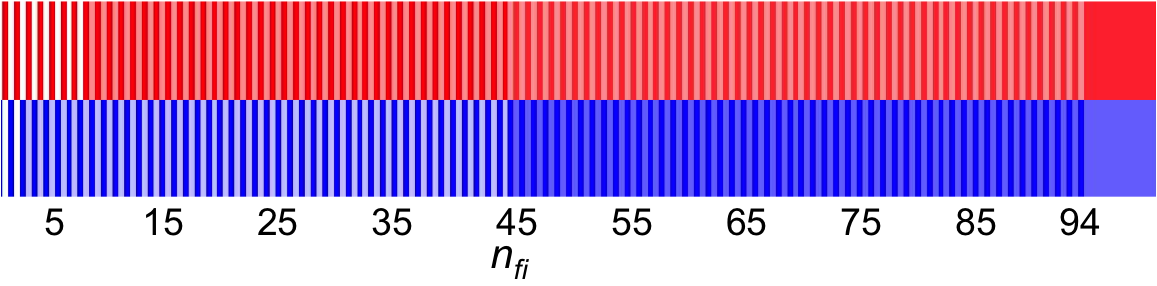
\includegraphics[width=0.85\linewidth]{TrainingData/figs/pt005proxdivAAO2.png} \\ 
(a) AAO approach with $\Delta=0.005$ \\ 
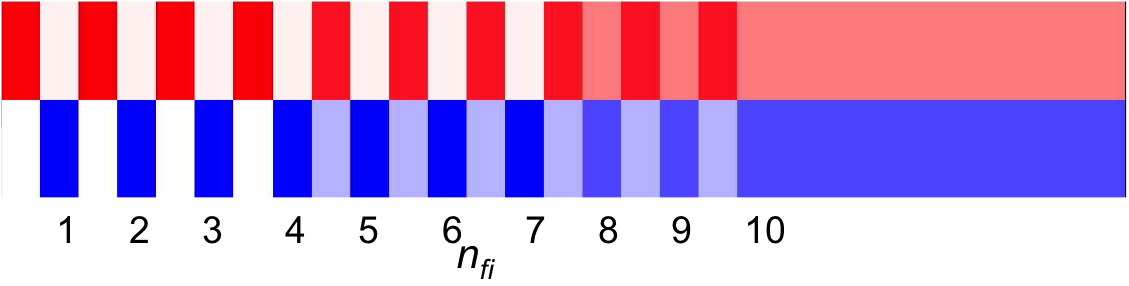
\includegraphics[width=0.85\linewidth]{TrainingData/figs/pt05proxdivAAO2.png} \\ 
(b) AAO approach with $\Delta=0.05$ \\ 
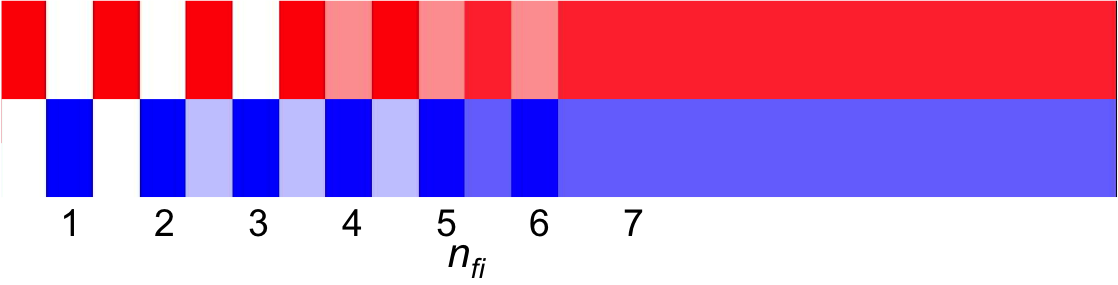
\includegraphics[width=0.85\linewidth]{TrainingData/figs/proxdivadaptAAO2.png} \\ 
(c) Adapt AAO approach 
\end{tabular} 
\caption{Variation in average proximity (red) and diversity (blue) of selected keywords for selecting 5 SRKs from 20 valid keywords of category ``$Baby$" using (a)  AAO with $\Delta=0.005$, (b) AAO with $\Delta=0.05$, and (c) Adapt AAO. Higher color intensity corresponds to a higher value of the corresponding objective function. $T$ increases along the X axis. Note that the range of variation in the two colors are different, and for both colors, white is assigned to the lowest value of the corresponding objective function value observed during the optimization. }
\label{fig:proxdivVariationAAO}
\end{figure*}


Since too large or small values of $\Delta$ lead to issues such as bias between objective functions, and large number of iterations taken for AAO approach to converge, we propose an adaptive approach that eliminates the need to have a fixed $\Delta$. Instead, the proposed approach updates $T$ based on the \textit{weakest permitted} algorithm iteration in the previous framework iteration whenever it detects repetitions in the selected keywords. The weakest permitted algorithm iteration is the algorithm iteration of either \textit{Max-Proximity} or \textit{Max-Diversity} with the least relative benefit that occurred in the previous framework iteration. Relative benefit has been defined for \textit{Max-Proximity} and \textit{Max-Diversity} algorithms in Section~\ref{sec:aaoproxmax} and Section~\ref{sec:aaodivmax} respectively. The adaptive annealing based alternating optimization (Adapt AAO) framework is presented in Algorithm~\ref{algo:AdaptAAO}. $WI_{Proximity}$ and $WI_{Diversity}$ represent the strength of the weakest permitted algorithm iteration permitted in the \textit{Max-Proximity} and \textit{Max-Diversity} algorithms respectively. Details on how $WI_{Proximity}$ and $WI_{Diversity}$ are computed in their respective algorithms are provided in Algorithms~\ref{algo:maxproximity} and \ref{algo:maxdiversity} respectively. Repetitions are detected in Algorithm~\ref{algo:AdaptAAO} when a set of selected keywords had been selected in a previous framework iteration.  


Based on the Adapt AAO approach, Fig.~\ref{fig:proxdivVariationAAO}(c) shows that the number of iterations taken to converge is much lower than in the case of $\Delta=0.005$ (Fig.~\ref{fig:proxdivVariationAAO}(a)). The resulting set of keywords is the same as in the case of $\Delta=0.005$, but with substantial reduction in number of iterations taken to converge (94 to 7). Since the Adapt AAO approach converges in significantly less framework iterations as compared to AAO, and does not result in any artificial bias towards an objective function, we only provide performance results based on Adapt AAO approach in Section~\ref{sec:expt}. 

\textbf{Complexity analysis for Algorithm~\ref{algo:AdaptAAO}.}
The \textit{Max-Proximity} algorithm (Algorithm~\ref{algo:maxproximity}) and the \textit{Max-Diversity} algorithm (Algorithm~\ref{algo:maxdiversity}) have worst-case complexities of $O(L^2 N_{Valid})$.  and $O(mL.N_{Valid})$ respectively. In each framework iteration, the two algorithms are run in alternation. Since $m > N_{Valid} > L$, the dominating number of computations is due to the term $O(mL.N_{Valid})$. Thus the total worst case time complexity of Algorithm~\ref{algo:AdaptAAO} is $O(mL.N_{Valid}N_{FrameworkIter})$ where $N_{FrameworkIter}$ is the number of framework iterations. 

